%%%%%%%%%%%%%%%%%%%%%%%%%%%%%%%%%%%%%%%%%%%%%%%%%%%%%%%%%%
\begin{frame}
  \begin{beamerboxesrounded}{}
	\begin{center}

\vspace{20pt}

		Architecture

\vspace{20pt}

	\end{center}    
  \end{beamerboxesrounded}
\end{frame}


%%%%%%%%%%%%%%%%%%%%%%%%%%%%%%%%%%%%%%%%%%%%%%%%%%%%%%%%%%
\subsection{Seek vs. Transfer}
%%%%%%%%%%%%%%%%%%%%%%%%%%%%%%%%%%%%%%%%%%%%%%%%%%%%%%%%%%
\frame {\frametitle{Seek vs. Transfer}
  \begin{itemize}
  \item \textbf{Fundamental difference between RDBMS and alternatives}
    \begin{itemize}
    \item B+Trees
    \item Log-Structured Merge Trees
    \end{itemize}

    \vspace{20pt}

  \item \textbf{Seek vs. Transfer}
    \begin{itemize}
    \item Random access to individual cells
    \item Sequential access to data
    \end{itemize}
  \end{itemize}
}

\frame {\frametitle{B+ Trees}
  \begin{itemize}
  \item \textbf{Dynamic, multi-level indexes}
    \begin{itemize}
    \item Efficient insertion, lookup and deletion
    \item {\color{red}Q: What's the difference between a B+ Tree and a
        Hash Table?}
    \item Frequent updates may imbalance the trees $\to$ Tree
      optimization and re-organization is required (which is a costly operation)
    \end{itemize}

    \vspace{20pt}

  \item \textbf{Bounds on \textit{page size}}
    \begin{itemize}
    \item Number of keys in each branch
    \item Larger fanout compared to binary trees
    \item Lower number of I/O operations to find a specific key
    \end{itemize}

    \vspace{20pt}

  \item \textbf{Support for range scans}
    \begin{itemize}
    \item Leaves are linked and represent an in-order list of all keys
    \item No costly tree-traversal algorithms required
    \end{itemize}
  \end{itemize}
}

\frame {\frametitle{LSM-Trees}
  \begin{itemize}
  \item \textbf{Data flow}
    \begin{itemize}
    \item Incoming data is first stored in a logfile,
      \textit{sequentially}
    \item Once the log has the modification saved, data is pushed in
      memory
      \begin{itemize}
    \item In-memory store holds most recent updates for fast lookup
      \end{itemize}
    \item When memory is ``full'', data is flushed in a store file to
      disk, as a sorted list of \texttt{key $\to$ record} pair
    \item At this point, the log file can be thrown away
    \end{itemize}

    \vspace{20pt}

  \item \textbf{How store files are arranged}
    \begin{itemize}
    \item Similar idea of a B+ Tree, but optimized for sequential disk
      access
    \item All nodes of the tree try to be filled up completely
    \item Updates are done in a \textbf{rolling merge} fashion
      \begin{itemize}
      \item The system packs existing on-disk multi-page blocks with
        in-memory data until the block reaches full capacity
      \end{itemize}
    \end{itemize}
  \end{itemize}
}

\frame {\frametitle{LSM-Trees}
  \begin{itemize}
  \item \textbf{Clean-up process}
    \begin{itemize}
    \item As flushes take place over time, a lot of store files are
      created
    \item Background process aggregates files into larger ones to
      limit disk seeks
    \item All store files are always sorted by key $\to$ no
      re-ordering required to fit new keys in
    \end{itemize}

    \vspace{20pt}

  \item \textbf{Data Lookup}
    \begin{itemize}
    \item Lookups are done in a merging fashion
      \begin{itemize}
      \item First lookup in the in-memory store
      \item If miss, the lookup in the on-disk store
      \end{itemize}
    \end{itemize}

    \vspace{20pt}

  \item \textbf{Deleting data}
    \begin{itemize}
    \item Use a \textit{delete marker}
    \item When pages are re-written, deleted markers and keys are
      eventually dropped
    \item Predicate deletion happens here
    \end{itemize}
  \end{itemize}
}

\frame {\frametitle{B+ Tree vs. LSM-Trees}
  \begin{itemize}
  \item \textbf{B+ Tree \cite{b+tree}}
    \begin{itemize}
    \item Work well when there are not so many updates
    \item The more and the faster you insert data at random locations
      the faster pages get fragmented
    \item \textbf{Updates and deletes are done at disk seek rates, rather than
      transfer rates}
    \end{itemize}

    \vspace{20pt}

  \item \textbf{LSM-Tree \cite{ONeil1996}}
    \begin{itemize}
    \item Work at disk transfer rate and scale better to huge amounts
      of data
    \item Guarantee a consistent insert rate
      \begin{itemize}
      \item They transform random into sequential writes
      \end{itemize}
    \item Reads are independent from writes
    \item Optimized data layout which offers predictable boundaries on
      disk seeks
    \end{itemize}
  \end{itemize}
}



%%%%%%%%%%%%%%%%%%%%%%%%%%%%%%%%%%%%%%%%%%%%%%%%%%%%%%%%%%
\subsection{Storage}
%%%%%%%%%%%%%%%%%%%%%%%%%%%%%%%%%%%%%%%%%%%%%%%%%%%%%%%%%%
\frame {\frametitle{Storage}
  \begin{beamerboxesrounded}{}
    Overview
  \end{beamerboxesrounded}
  \begin{figure}[h]
    \centering
    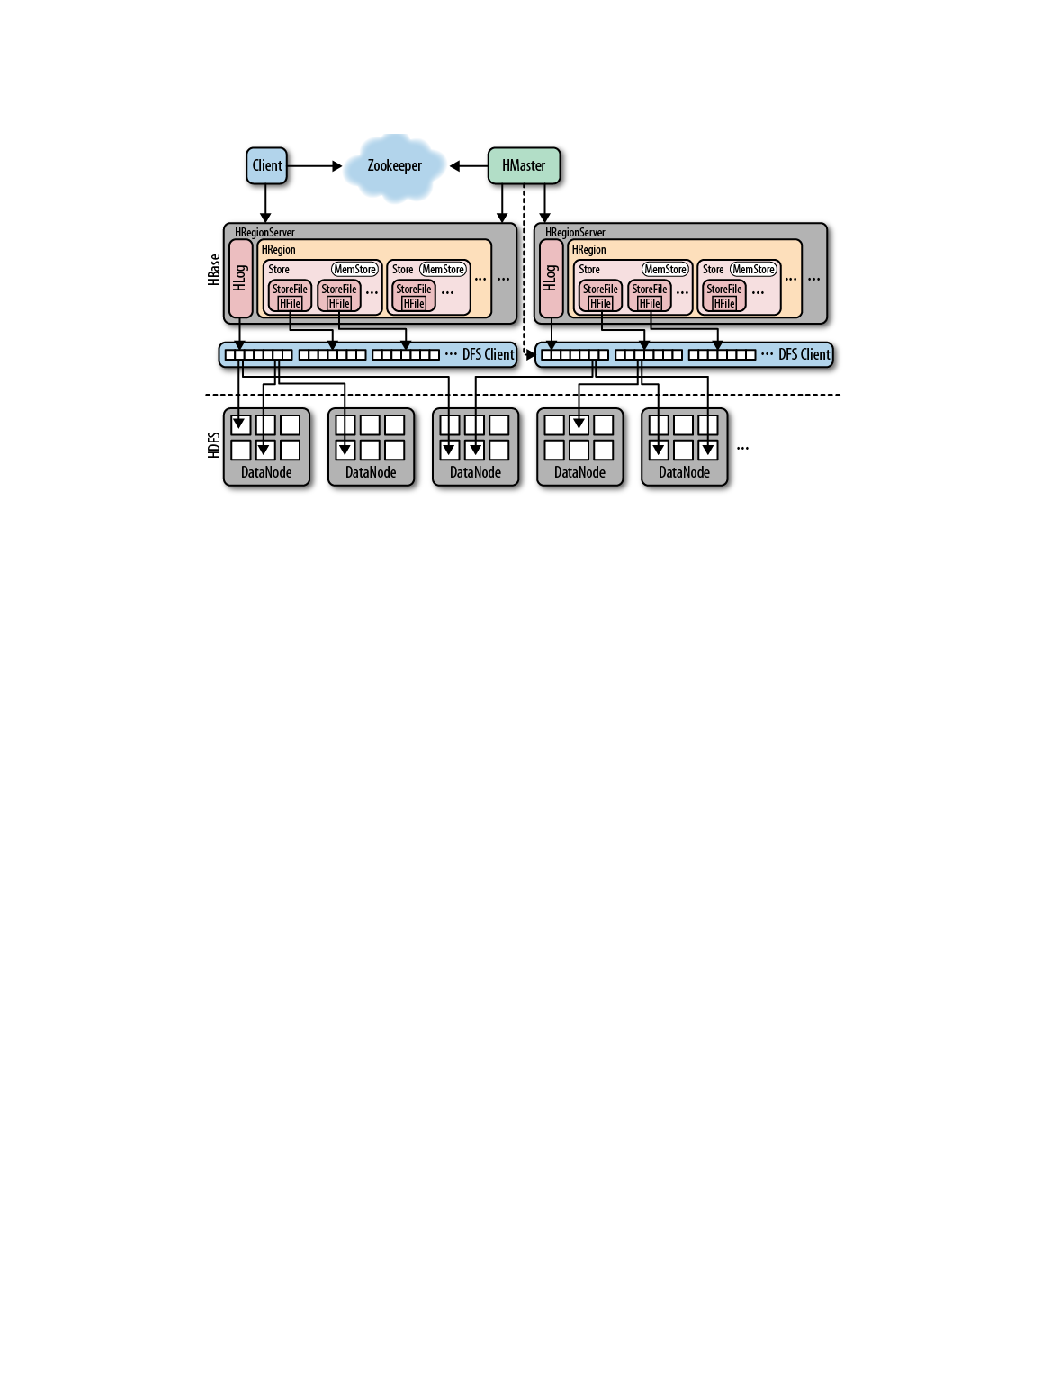
\includegraphics[scale=0.9]{./figures/hbase-storage}
    \caption{Overview of how HBase handles files in the filesystem}
    \label{fig:hbase-storage}
  \end{figure}
}

\frame {\frametitle{Storage}
  \begin{beamerboxesrounded}{}
    Overview
  \end{beamerboxesrounded}

  \begin{itemize}
  \item \textbf{HBase handles two kinds of file types}
    \begin{itemize}
    \item One is used for the WAL
    \item One is used for the actual data storage
    \end{itemize}

    \vspace{20pt}

  \item \textbf{Who does what}
    \begin{itemize}
    \item \texttt{HMaster}
      \begin{itemize}
      \item Low-level operations
      \item Assigns region servers to key space
      \item Keeps metadata
      \item Talks to ZooKeeper
      \end{itemize}
    \item \texttt{HRegionServer}
      \begin{itemize}
      \item Handles the WAL and \texttt{HFiles}
      \item These files are divided in to blocks and stored into HDFS
      \item Block size is a parameter
      \end{itemize}
    \end{itemize}

  \end{itemize}
}

\frame {\frametitle{Storage}
  \begin{beamerboxesrounded}{}
    Overview
  \end{beamerboxesrounded}

  \begin{itemize}
  \item \textbf{General communication flow}
    \begin{itemize}
    \item A client contacts ZooKeeper when trying to access a
      particular row
    \item Recovers from ZooKeeper the server name that host the
      \texttt{-ROOT-} region
    \item Using the \texttt{-ROOT-} information the client retrieves
      the server name that host the \texttt{.META.} table region
      \begin{itemize}
      \item The \texttt{.META.} table region contains the row key in question
      \end{itemize}
    \item Contact the reported \texttt{.META.} server and retrieve the
      server name that has the region containing the row key in question
    \end{itemize}

    \vspace{20pt}

  \item \textbf{Caching}
    \begin{itemize}
    \item Generally, lookup procedures involve caching row key
      locations for faster subsequent lookups
    \end{itemize}
  \end{itemize}
}

\frame {\frametitle{Storage}
  \begin{beamerboxesrounded}{}
    Overview
  \end{beamerboxesrounded}

  \begin{itemize}
  \item \textbf{Important Java Classes}
    \begin{itemize}
    \item \texttt{HRegionServer} handles one or more regions and
      create the corresponding \texttt{HRegion} object
    \item When an \texttt{HRegion} object is opened it creates
      a \texttt{Store} instance for each \texttt{HColumnFamily}
    \item Each \texttt{Store} instance can have:
      \begin{itemize}
      \item One or more \texttt{StoreFile} instances
      \item A \texttt{MemStore} instance
      \end{itemize}
    \item \texttt{HRegionServer} has a shared \texttt{HLog} instance
    \end{itemize}
  \end{itemize}
}

\frame {\frametitle{Storage}
  \begin{beamerboxesrounded}{}
    Write Path
  \end{beamerboxesrounded}

  \begin{itemize}
  \item \textbf{External client insert data in HBase}
    \begin{itemize}
    \item Issues an \texttt{HTable.put(Put)} request to \texttt{HRegionServer}
    \item \texttt{HRegionServer} hands the request to the \texttt{HRegion} instance that
      matches the request [{\color{red}Q: What is the matching criteria?}]
    \end{itemize}

    \vspace{20pt}

  \item \textbf{How the system reacts to a write request}
    \begin{itemize}
    \item Write data to the WAL, represented by the \texttt{HLog}
      class
      \begin{itemize}
      \item The WAL stores \texttt{HLogKey} instances in a HDFS
        \texttt{SequenceFile}
      \item These keys contain a sequence number and the actual data
      \item In case of failure, this data can be used to replay
        not-yet-persisted data
      \end{itemize}
    \item Copy data in the \texttt{MemStore}
      \begin{itemize}
      \item Check if MemStore size has reached a threshold
      \item If yes, launch a \textit{flush request}
      \item Launch a thread in the \texttt{HRegionServer} and flush \texttt{MemStore} data
        to an \texttt{HFile}
      \end{itemize}
    \end{itemize}
  \end{itemize}
}

\frame {\frametitle{Storage}
  \begin{beamerboxesrounded}{}
    HBase Files
  \end{beamerboxesrounded}

  \begin{itemize}
  \item \textbf{What and where are HBase files (including WAL,
    \texttt{HFile},...) stored?}
    \begin{itemize}
    \item HBase has a root directory set to ``\texttt{/hbase}'' in
      HDFS
    \item Files can be divided into:
      \begin{itemize}
      \item Those that reside under the HBase root directory
      \item Those that are in the \textit{per-table} directories
      \end{itemize}
    \end{itemize}

    \vspace{20pt}

  \item \texttt{/hbase}
    \begin{itemize}
    \item \texttt{.logs}
    \item \texttt{.oldlogs}
    \item \texttt{.hbase.id}
    \item \texttt{.hbase.version}
    \item \texttt{/example-table}
    \end{itemize}
  \end{itemize}
}

\frame {\frametitle{Storage}
  \begin{beamerboxesrounded}{}
    HBase Files
  \end{beamerboxesrounded}
  
  \begin{itemize}
  \item \texttt{/example-table}
    \begin{itemize}
    \item \texttt{.tableinfo}
    \item \texttt{.tmp}
    \item \texttt{``\texttt{...Key1...}''}
      \begin{itemize}
      \item \texttt{.oldlogs}
      \item \texttt{.regioninfo}
      \item \texttt{.tmp}
      \item \texttt{colfam1/}
      \end{itemize}
    \end{itemize}

  \item \texttt{colfam1/}
    \begin{itemize}
    \item ``\texttt{....column-key1...}''
    \end{itemize}
  \end{itemize}
}

\frame {\frametitle{Storage}
  \begin{beamerboxesrounded}{}
    HBase: Root-level files
  \end{beamerboxesrounded}

  \begin{itemize}
  \item \textbf{\texttt{.logs} directory}
    \begin{itemize}
    \item WAL files handled by \texttt{HLog} instances
    \item Contains a subdir for each \texttt{HRegionServer}
    \item Each subdir contains many \texttt{HLog} files
    \item All regions from that \texttt{HRegionServer} share the same
      HLog files
    \end{itemize}
  \item \texttt{.oldlogs} directory
    \begin{itemize}
    \item When data is persisted to disk (from \texttt{Memstores}) log
      files are decommissioned to the \texttt{.oldlogs} dir
    \end{itemize}

    \vspace{20pt}

  \item \textbf{\texttt{hbase.id} and \texttt{hbase.version}}
    \begin{itemize}
    \item Represent the unique ID of the cluster and the file format version
    \end{itemize}
  \end{itemize}
}

\frame {\frametitle{Storage}
  \begin{beamerboxesrounded}{}
    HBase: Table-level files
  \end{beamerboxesrounded}

  \begin{itemize}
  \item \textbf{Every table has its own directory}
    \begin{itemize}
    \item \texttt{.tableinfo}: stores the serialized
      \texttt{HTableDescriptor}
      \begin{itemize}
      \item This include the table and column family schema
      \end{itemize}
    \item \texttt{.tmp} directory
      \begin{itemize}
      \item Contains temporary data
      \end{itemize}
    \end{itemize}
  \end{itemize}
}

\frame {\frametitle{Storage}
  \begin{beamerboxesrounded}{}
    HBase: Region-level files
  \end{beamerboxesrounded}

  \begin{itemize}
  \item \textbf{Inside each table dir, there is a separate dir for every
      region in the table}
    \begin{itemize}
    \item The name of each of these dirs is the MD5 hash of a region name
      \begin{itemize}
      \item Inside each region there is a directory for each column
        family
      \item Each column family directory holds the actual data files,
        namely \texttt{HFiles}
      \item Their name is just an arbitrary random number
      \end{itemize}
    \item Each region directory also has a \texttt{.regioninfo} file
      \begin{itemize}
      \item Contains the serialized information of the \texttt{HRegionInfo} instance
      \end{itemize}
    \end{itemize}
    
    \vspace{20pt}
    
  \item \textbf{Split Files}
    \begin{itemize}
    \item Once the region needs to be split, a \texttt{splits}
      directory is created
      \begin{itemize}
      \item This is used to stage two daughter regions
      \item If split is successful, daughter regions are moved up to
        the table directory
      \end{itemize}
    \end{itemize}
  \end{itemize}
}

\frame {\frametitle{Storage}
  \begin{beamerboxesrounded}{}
    HBase: A note on region splits
  \end{beamerboxesrounded}

  \begin{itemize}
  \item \textbf{Splits triggered by store file (region) size}
    \begin{itemize}
    \item Region is split in two
    \item Region is closed to new requests
    \item \texttt{.META.} is updated
    \end{itemize}
    
    \vspace{20pt}
    
  \item \textbf{Daughter regions initially reside on the same server}
    \begin{itemize}
    \item Both daughters are compacted
    \item Parent is cleaned up
    \item \texttt{.META.} is updated
    \end{itemize}
    
    \vspace{20pt}
    
  \item \textbf{Master schedules new regions to be moved off to other servers}
  \end{itemize}  
}

\frame {\frametitle{Storage}
  \begin{beamerboxesrounded}{}
    HBase: Compaction
  \end{beamerboxesrounded}

  \begin{itemize}
  \item \textbf{Process that takes care of re-organizing store files}
    \begin{itemize}
    \item Essentially to conform to underlying filesystem requirements
    \item Compaction check when memstore is flushed
    \end{itemize}

    \vspace{20pt}

  \item \textbf{Minor and Major compactions}
    \begin{itemize}
    \item Always from the oldest to the newest files
    \item Avoid all servers to perform compaction concurrently
    \end{itemize}
  \end{itemize}

  \begin{figure}[h]
    \centering
    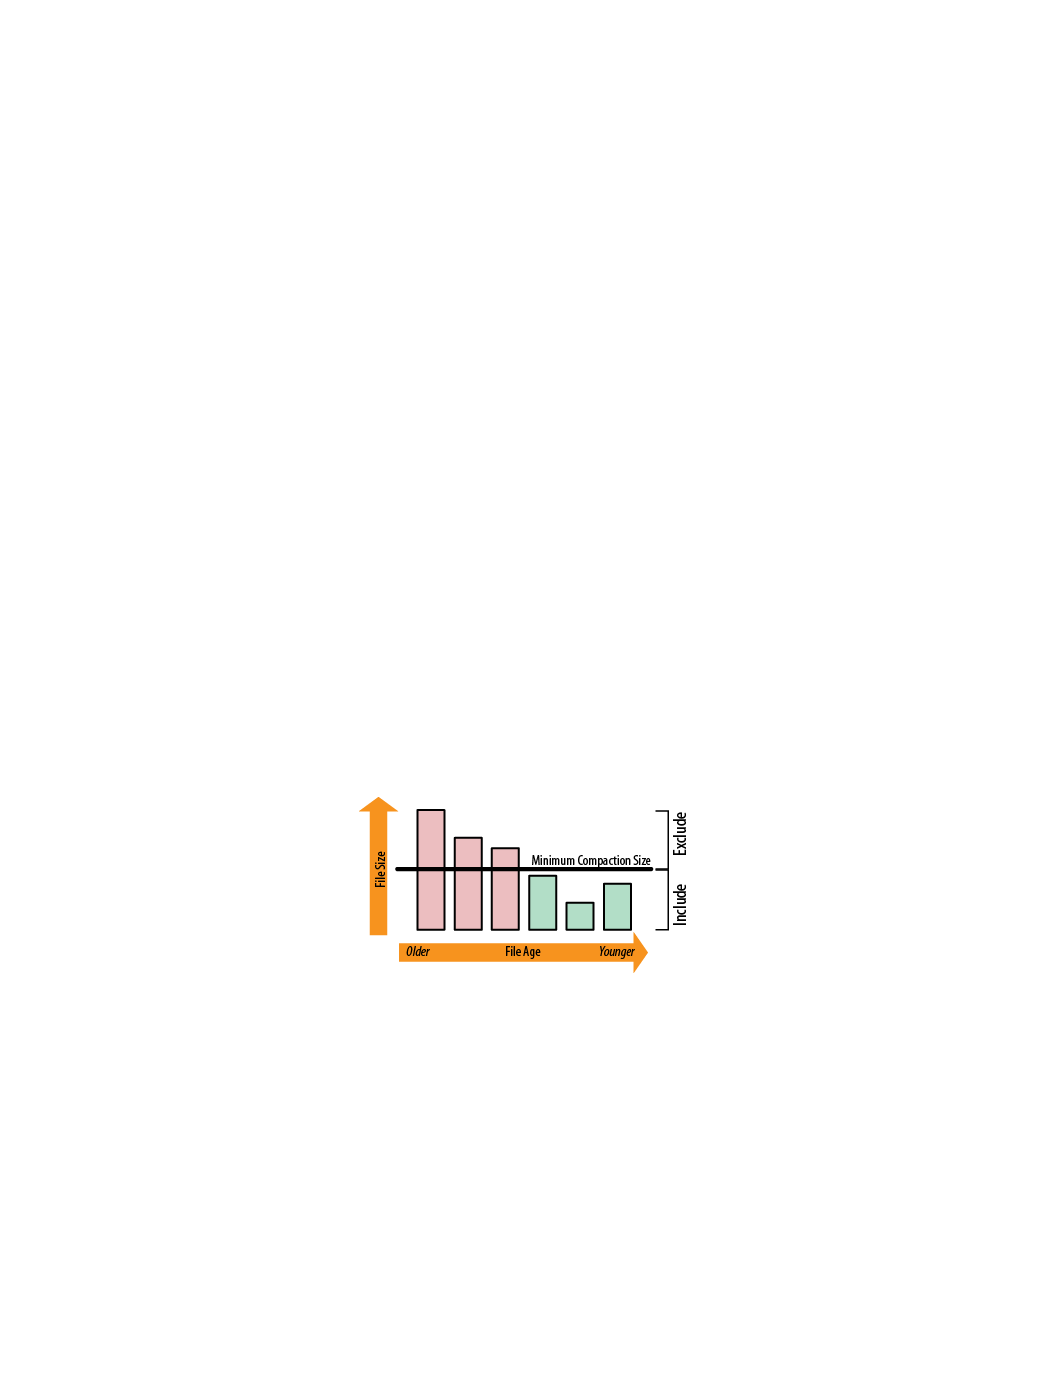
\includegraphics[scale=0.7]{./figures/compaction}
    \caption{A set of store files showing the minimum compaction threshold}
    \label{fig:compaction}
  \end{figure}
}

\frame {\frametitle{Storage}
  \begin{beamerboxesrounded}{}
    HFile format
  \end{beamerboxesrounded}

  \begin{itemize}
  \item \textbf{Store files are implemented by the \texttt{HFile} class}
    \begin{itemize}
    \item Efficient data storage is the goal
    \end{itemize}

    \vspace{20pt}

  \item \textbf{\texttt{HFiles} consist of a variable number of
      blocks}
    \begin{itemize}
    \item Two fixed blocks: \textit{info} and \textit{trailer}
    \item \textit{index} block: records the offsets of the \texttt{data} and
      meta \texttt{blocks}
    \item Block size: \textit{large} $\to$ sequential access; \textit{small} $\to$
      random access
    \end{itemize}
  \end{itemize}

  \begin{figure}[h]
    \centering
    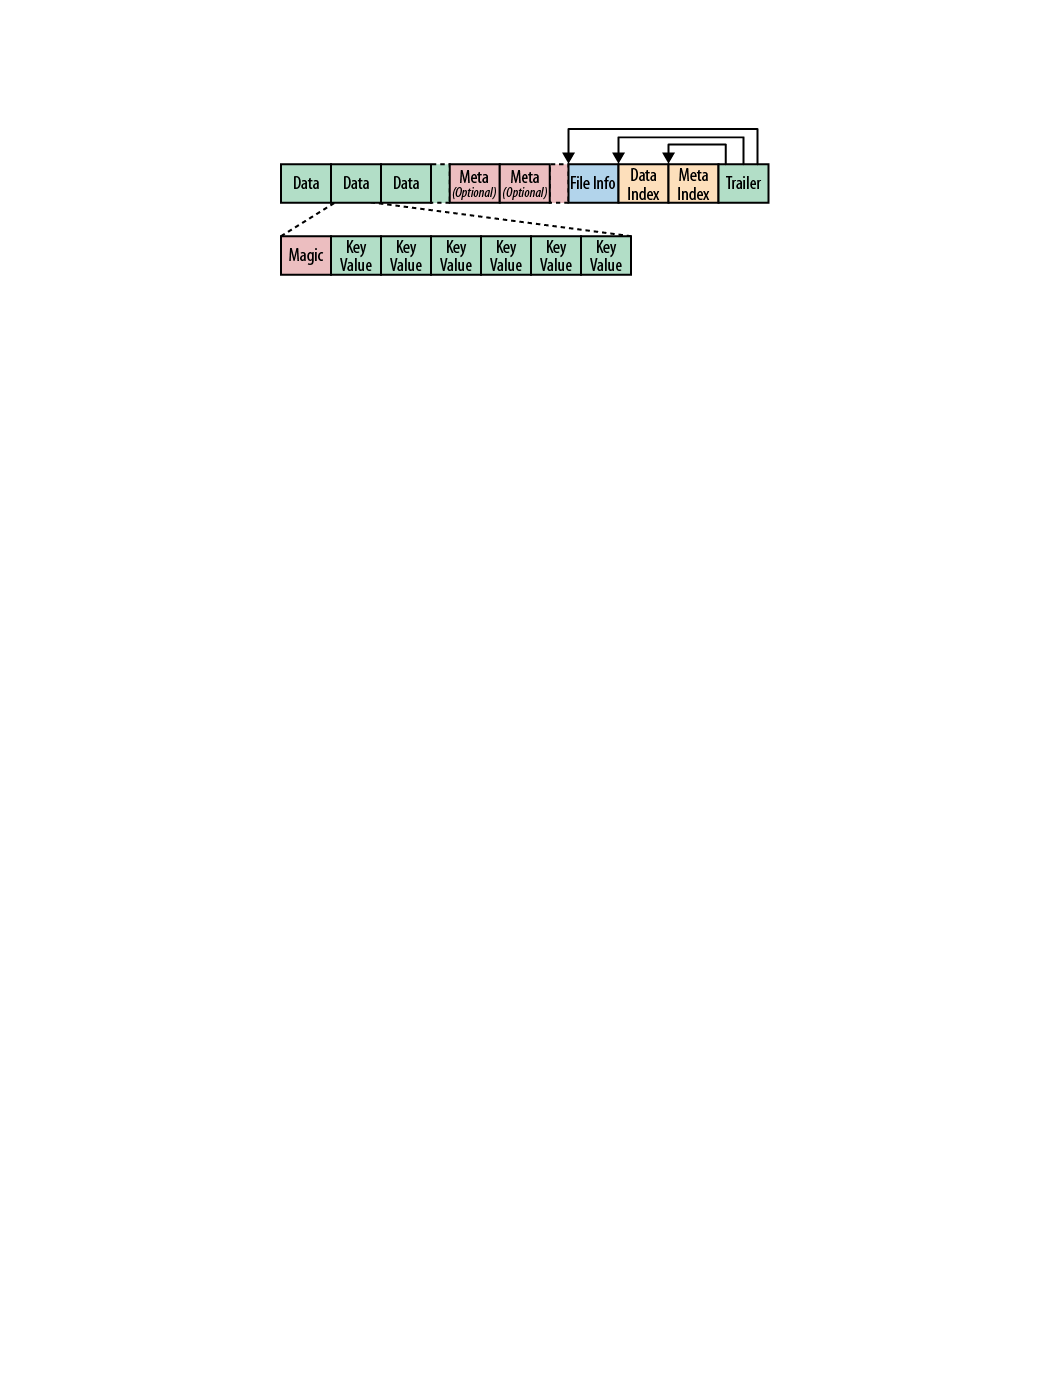
\includegraphics[scale=0.8]{./figures/hfile}
    \caption{The HFile structure}
    \label{fig:hfile}
  \end{figure}
}

\frame {\frametitle{Storage}
  \begin{beamerboxesrounded}{}
    HFile size and HDFS block size
  \end{beamerboxesrounded}

  \begin{itemize}
  \item \textbf{HBase uses any underlying filesystem}

    \vspace{20pt}

  \item \textbf{In case HDFS is used}
    \begin{itemize}
    \item HDFS block size is generally 64MB
    \item This is 1,024 times the default \texttt{HFile} block size
      (64 KB)
    \item[$\to$] There is no correlation between HDFS block and HFile sizes
    \end{itemize}
  \end{itemize}
}

\frame {\frametitle{Storage}
  \begin{beamerboxesrounded}{}
    The KeyValue Format
  \end{beamerboxesrounded}

  \begin{itemize}
  \item \textbf{Each KeyValue in the HFile is a low-level byte array}
    \begin{itemize}
    \item It allows for \textit{zero-copy} access to the data
    \end{itemize}

    \vspace{20pt}

  \item \textbf{Format}
    \begin{itemize}
    \item Fixed-length preambule indicates the length of the key and
      value
      \begin{itemize}
      \item This is useful to offset into the array to get direct
        access to the value, ignoring the key
      \end{itemize}
    \item Key format
      \begin{itemize}
      \item Contains row key, column family name, column qualifier...
      \item \texttt{[TIP]}: consider small keys to avoid overhead when storing
        small data
      \end{itemize}
    \end{itemize}
  \end{itemize}

  \begin{figure}[h]
    \centering
    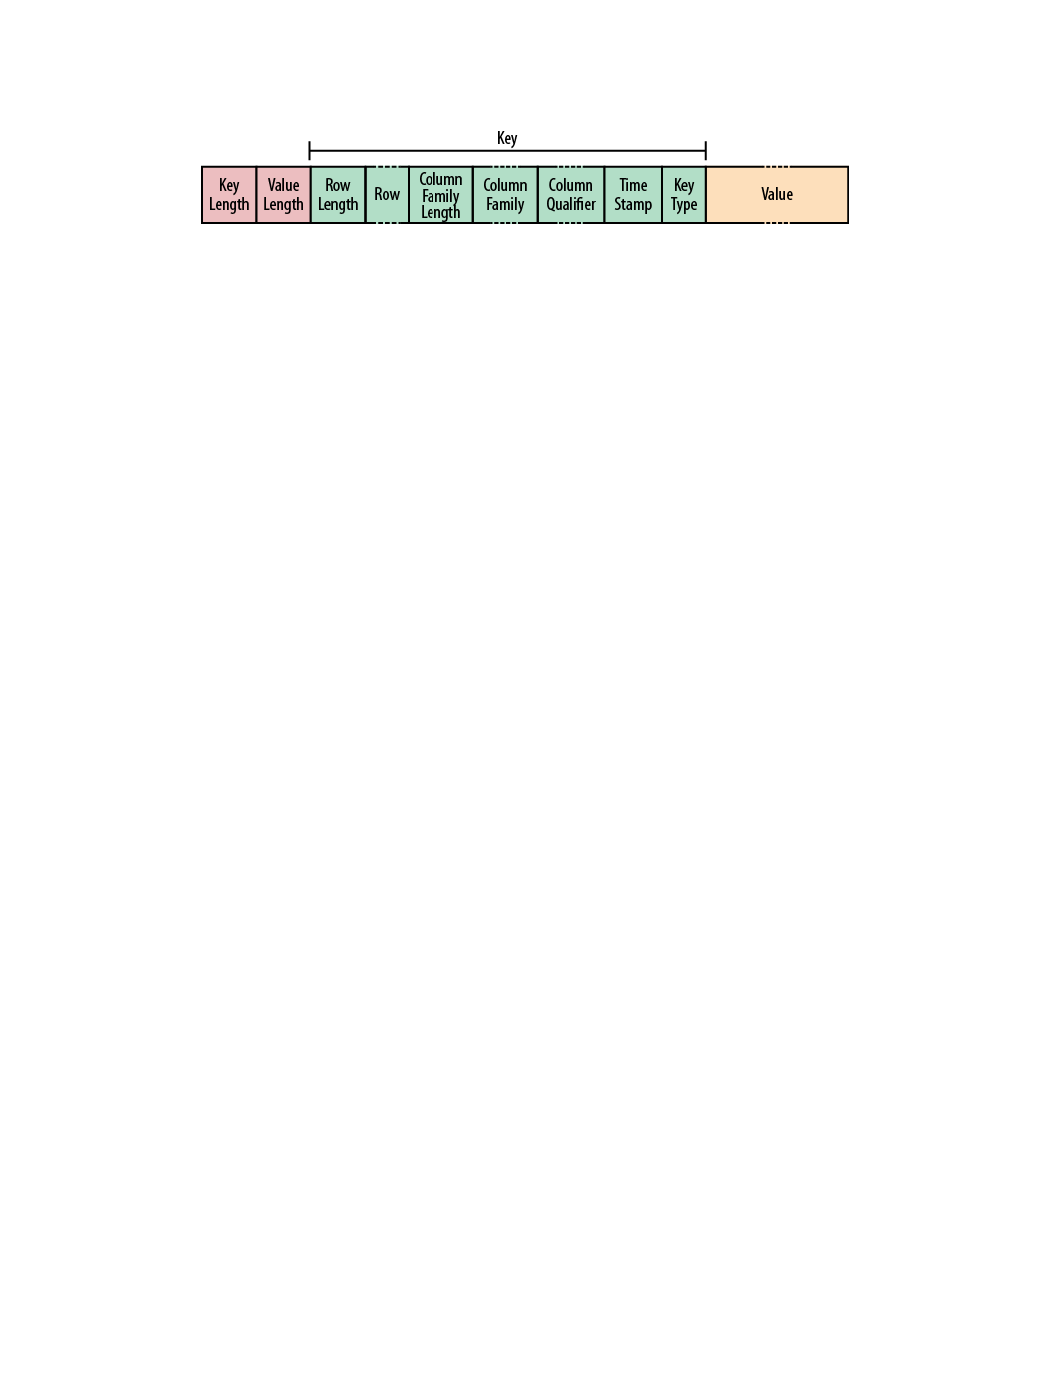
\includegraphics[scale=0.8]{./figures/keyvalue}
    \caption{The KeyValue Format}
    \label{fig:keyvalue}
  \end{figure}


}

%%%%%%%%%%%%%%%%%%%%%%%%%%%%%%%%%%%%%%%%%%%%%%%%%%%%%%%%%%
\subsection{WAL}
%%%%%%%%%%%%%%%%%%%%%%%%%%%%%%%%%%%%%%%%%%%%%%%%%%%%%%%%%%
\frame {\frametitle{The Write-Ahead Log}

  \begin{itemize}
  \item \textbf{Main tool to ensure resiliency to failures}
    \begin{itemize}
    \item Region servers keep data in-memory until enough is collected
      to warrant a flush
    \item What if the server crashes or power is lost?
    \end{itemize}

    \vspace{20pt}

  \item \textbf{WAL is a common approach to address fault-tolerance}
    \begin{itemize}
    \item Every data update is first written to a log
    \item Log is persisted (and replicated, since it resides on HDFS)
    \item Only when log is written, client is notified a successful
      operation on data
    \end{itemize}
  \end{itemize}

}

\frame {\frametitle{The Write-Ahead Log}

  \begin{figure}[h]
    \centering
    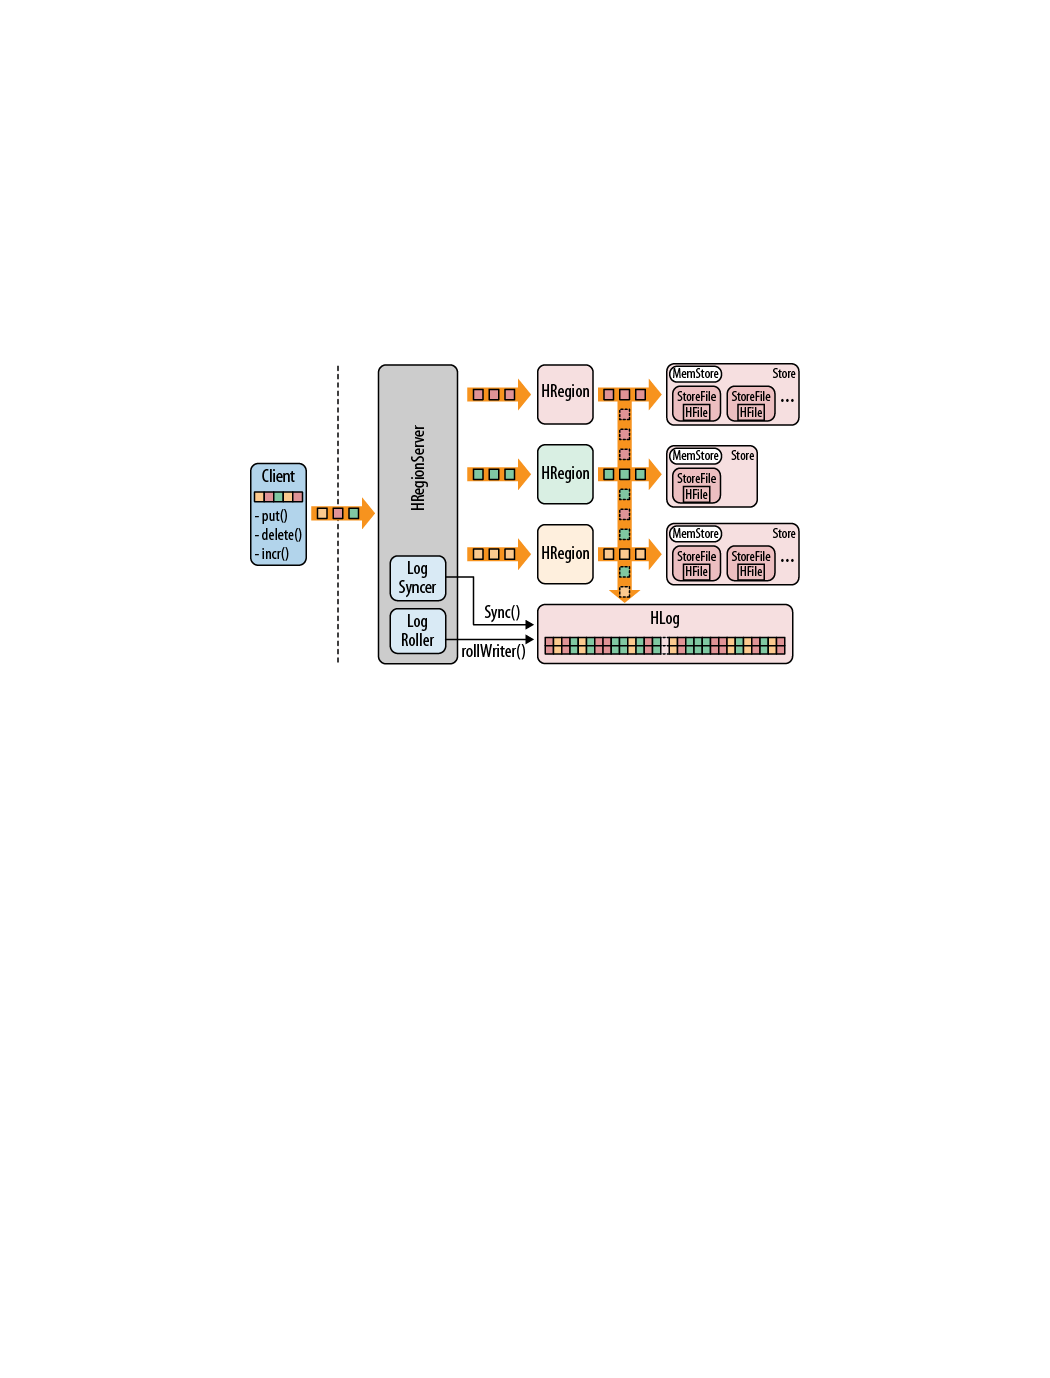
\includegraphics[scale=0.8]{./figures/wal}
    \caption{The write path of HBase}
    \label{fig:wal}
  \end{figure}

  \begin{itemize}
  \item \textbf{WAL records all changes to data}
    \begin{itemize}
    \item Can be replayed in case of server failure
    \item If write to WAL fails, the whole operations has to fail
    \end{itemize}
  \end{itemize}
}

\frame {\frametitle{The Write-Ahead Log}

  \begin{figure}[h]
    \centering
    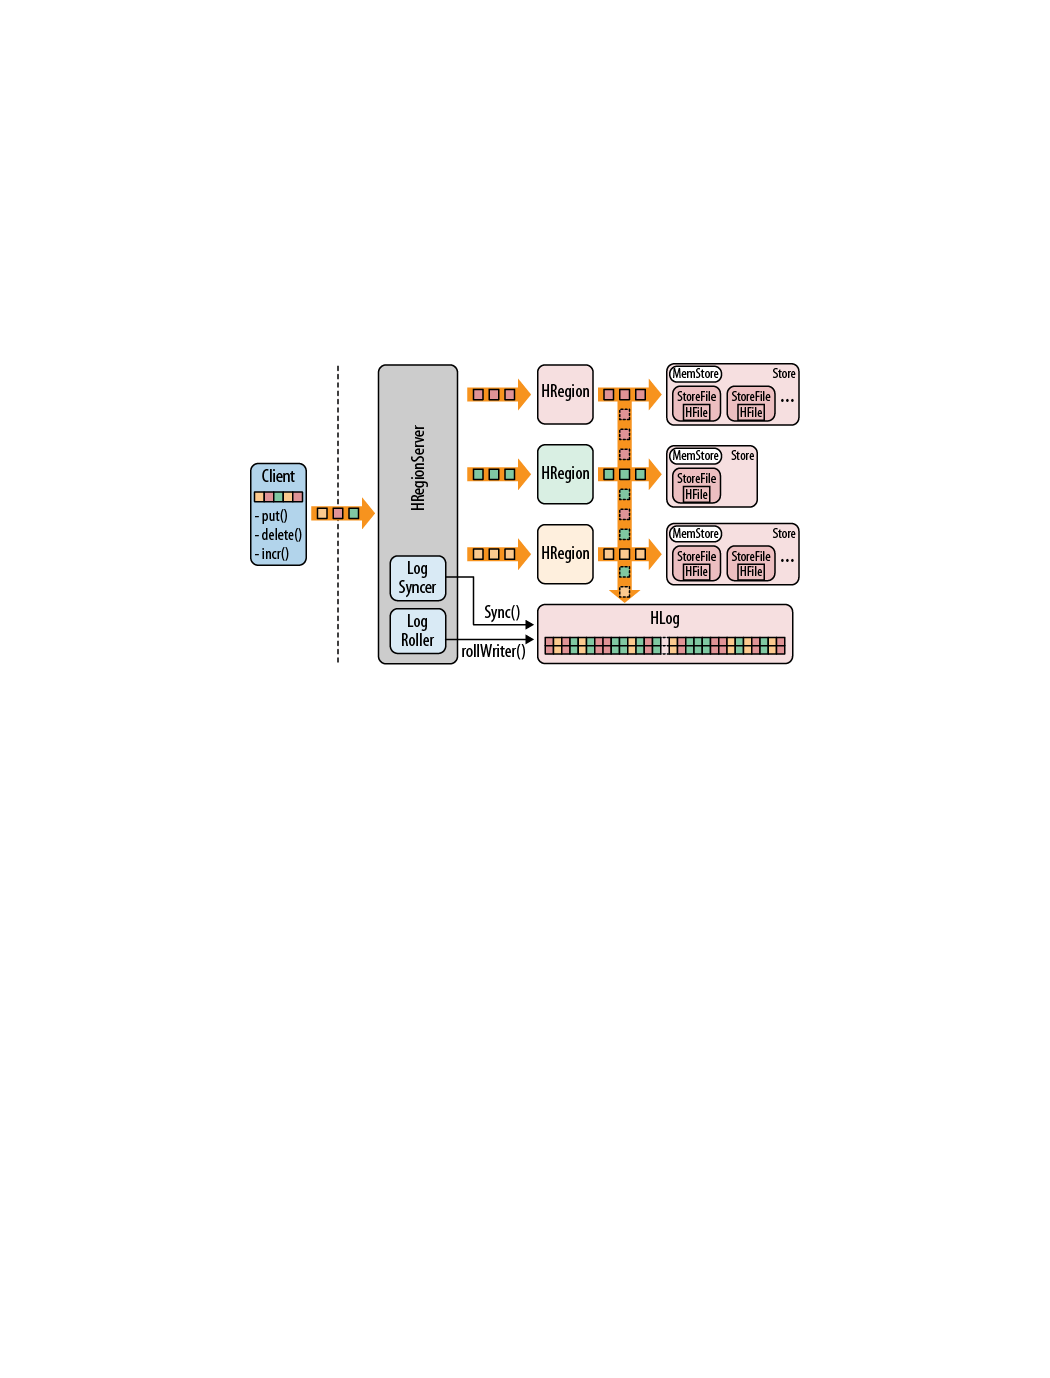
\includegraphics[scale=0.8]{./figures/wal}
  \end{figure}

  \begin{itemize}
  \item \textbf{Write Path}
    \begin{itemize}
    \item Client modifies data (\texttt{put()}, \texttt{delete()},
      \texttt{increment()})
    \item Modifications are wrapped into a KeyValue object
    \item Objects are batched to the corresponding
      \texttt{HRegionServer}
    \item Objects are routed to the corresponding \texttt{HRegion}
    \item Objects are written to WAL and in the \texttt{MemStore}
    \end{itemize}
  \end{itemize}
}


%%%%%%%%%%%%%%%%%%%%%%%%%%%%%%%%%%%%%%%%%%%%%%%%%%%%%%%%%%
\subsection{Read Path}
%%%%%%%%%%%%%%%%%%%%%%%%%%%%%%%%%%%%%%%%%%%%%%%%%%%%%%%%%%
\frame {\frametitle{Read Path}
  \begin{itemize}
  \item \textbf{HBase uses multiple store files per column family}
    \begin{itemize}
    \item These can be either in-memory and/or materialized on disk
    \item Compactions and clean-up background processes take care of
      store files maintenance
    \item Store files are immutable, so deletion is handled in a
      special way
    \end{itemize}

    \vspace{20pt}

  \item \textbf{The anatomy of a \texttt{get} command}
    \begin{itemize}
    \item HBase uses a \texttt{QueryMatcher} in combination with a
      \texttt{ColumnTracker}
    \item First, an exclusion check is performed to filter skip files
      (and eventually tombstone labelled data)
    \item Scanning data is implemented by a \texttt{RegionScanner}
      class which retrieves a \texttt{StoreScanner}
    \item \texttt{StoreScanner} includes both the \texttt{MemStore}
      and \texttt{HFiles}
    \item Read/Scans happen in the same order as data is saved
    \end{itemize}
  \end{itemize}
}

%%%%%%%%%%%%%%%%%%%%%%%%%%%%%%%%%%%%%%%%%%%%%%%%%%%%%%%%%%
\subsection{Region Lookups}
%%%%%%%%%%%%%%%%%%%%%%%%%%%%%%%%%%%%%%%%%%%%%%%%%%%%%%%%%%
\frame {\frametitle{Region Lookups}
  \begin{itemize}
  \item \textbf{How does a client find the region server hosting a specific
      row key range?}
    \begin{itemize}
    \item HBase uses two special catalog tables, \texttt{-ROOT-} and
      \texttt{.META.}
    \item The \texttt{-ROOT-} table is used to refer to all regions in the
      \texttt{.META.} table
    \end{itemize}
    
    \vspace{20pt}
    
  \item \textbf{Three-level B+ Tree -like operation}
    \begin{itemize}
    \item Level 1: a node stored in ZooKeeper, containing the location
      (region server) of the \texttt{-ROOT-} table
    \item Level 2: Lookup in the -ROOT- table to find a matching meta
      region
    \item Level 3: Retrieve the table region from the \texttt{.META.} table
    \end{itemize}
  \end{itemize}
}

\frame {\frametitle{Region Lookups}
  \begin{itemize}
  \item \textbf{Where to send requests when looking for a specific row
      key?}
    \begin{itemize}
    \item This information is cached, but the first time or when the
      cache is stale or when there is a miss due to compaction, the
      following procedure applies
    \end{itemize}

    \vspace{20pt}

  \item \textbf{Recursive discovery process}
    \begin{itemize}
    \item Ask the region server hosting the matching \texttt{.META.}
      table to retrieve the row key address
    \item If the information is invalid, it backs out: asks the
      \texttt{-ROOT-} table where the relevant \texttt{.META.} region
      is
    \item If this fails, ask ZooKeeper where the \texttt{-ROOT-} table is
    \end{itemize}
  \end{itemize}
}

\frame {\frametitle{Region Lookups}
  \begin{figure}[h]
    \centering
    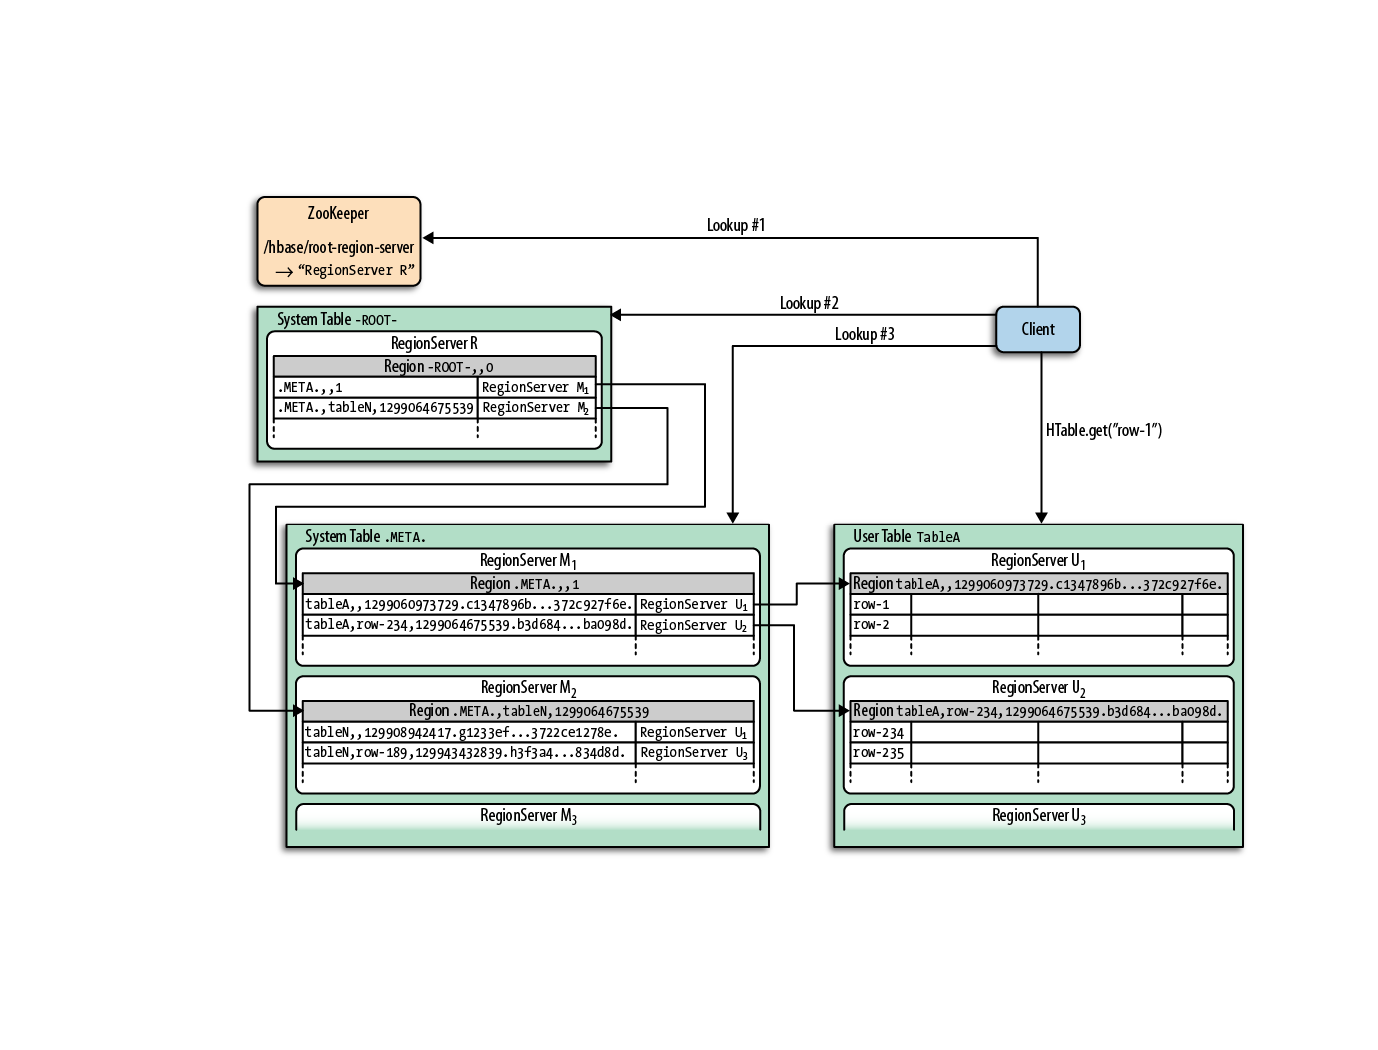
\includegraphics[scale=0.6]{./figures/lookup}
  \end{figure}
}